\section{Interface Research}
As a social network, the user interface design is of high importance, as a lot 
of users of the program will have little core system knowledge, and rely 
entirely on the user interface. As a result we have looked at a variety of 
options into designing which will be the best for the project.

\subsection{Swing}
Swing is the primary Java GUI toolkit, providing a basic standpoint for entry 
level interface designing. Introduced back in 1996, Swing was designed to be 
an interface style that required minimal changes to the applications code, 
providing the user with a pluggable look and feel mechanism. It has been apart 
of the standard java library for over a decade, which, as I will now explain, 
may not be to our benefit.

Swing, whilst an excellent language to begin with, and write simple applications
in, is quite dated. As our group advisor put it when inquiring about what we 
would be coding the user interface in:

\begin{quote}
"You should avoid Swing to prevent it looking like it was done in the 
nineties." - Sebastian Coope
\end{quote}

Sebastian is not wrong either, as Swing does a very plain feel to it. This figure 
shows an old instant messaging system written with Swing by one of our team 
members. As you can see it is unlikely to appeal to the mass market with such 
visually plain appearance. This makes Swing, unlikely to be our GUI toolkit of 
choice, despite some of our members experience with it.

\begin{figure}[h]
    \centering
    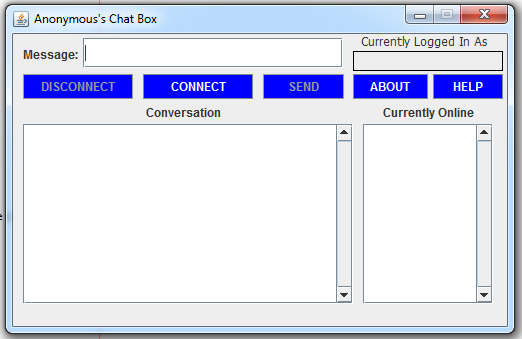
\includegraphics[width=\textwidth]{images/design/swing.jpg}
    \caption{Swing Instant Messaging Application}
    \label{fig:swing_im}
\end{figure}

\subsection{Abstract Window Toolkit}
Abstract Window Toolkit (otherwise known as AWT), was another choice given 
that we are programming in Java, and synchronicity between the two would be an 
advantage. Whilst AWT retained some advantages such as its style blending in 
with each operating system it runs on, it is even older than Swing being Java's 
original toolkit, making any GUI displayed via it look rather dated. None of the
the current team has any proficiency with AWT however, and whilst it is 
possible to learn, there are still other options to consider that may provide 
the use with a more professional GUI build.

\subsection{Standard Widget Toolkit}
Standard Widget Toolkit (otherwise known as SWT), is one of the more promising 
candidates so far given its look and up-to-date support packages. The latest 
stable release of SWT was only last year, and is capable of producing programs 
with a modern and professionally built appearance, as shown in the figure.

\begin{figure}[H]
    \centering
    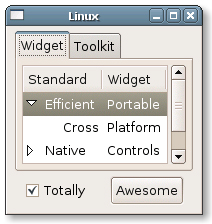
\includegraphics[width=\textwidth]{images/design/swt.jpg}
    \caption{SWT Appearance Style}
    \label{fig:swt_style}
\end{figure}

Unlike both Swing and AWT, SWT is not provided by Sun Microsystems as a part of 
the Java platform. It is now provided and maintained by the Eclipse Foundation, 
and provided as a part of their widely used Eclipse IDE, something a lot of the 
team is familiar with.

\subsection{GWT}
GWT allows you to create HTML/Javascript based user interfaces for Java 
applications running locally. The interface is programmed in Java and then GWT 
creates valid HTML/Javascript automatically. A web server is required in order
for Javascript events to be sent to the Java application.

The user can then interact with the system by pointing their web browser at 
localhost. This has the benefit of being familiar to novice users as most modern 
computer interaction is done within a web browser. 

Another advantage of using GWT is the ability to alter the appearance of web 
pages using CSS. This facilitates the creation of a modern, attractive user 
interface that integrates nicely with current operating systems and software.

\subsection{Javascript}
It is possible to create the entire client application in Javascript and use a 
HTML/Javascript GUI. This approach removes the need for a local web server 
meaning the only software the user is required to run is a modern web browser.

Another advantage would be tight integration between the logic and interface 
elements of the client application and no risk of errors caused by using 
multiple programming languages.

One disadvantage of this approach is the difficulty in implementing the
required security measures and encryption in Javascript. This can be remedied by 
using a Javascript library such as the Forge project which implements many 
cryptography methods.

The main disadvantage is that in this approach the server operator has complete
control of the client the user uses. This is unacceptable because we're assuming
that the server operator is seeking to spy on the user.

\section{GUI Design}
\subsection{Client Design}
Arguably the most important GUI in the project is the client GUI, as this is what
the standard user will be interacting with, a person whom we are assuming has no
knowledge of any inner workings. All tests we perform on our system at a later 
stage will be through this client, as per such its design takes a high level of
importance. Its for this reason we have chosen something common users will be 
more accustomed to; web pages.

\begin{figure}[h]
    \centering
    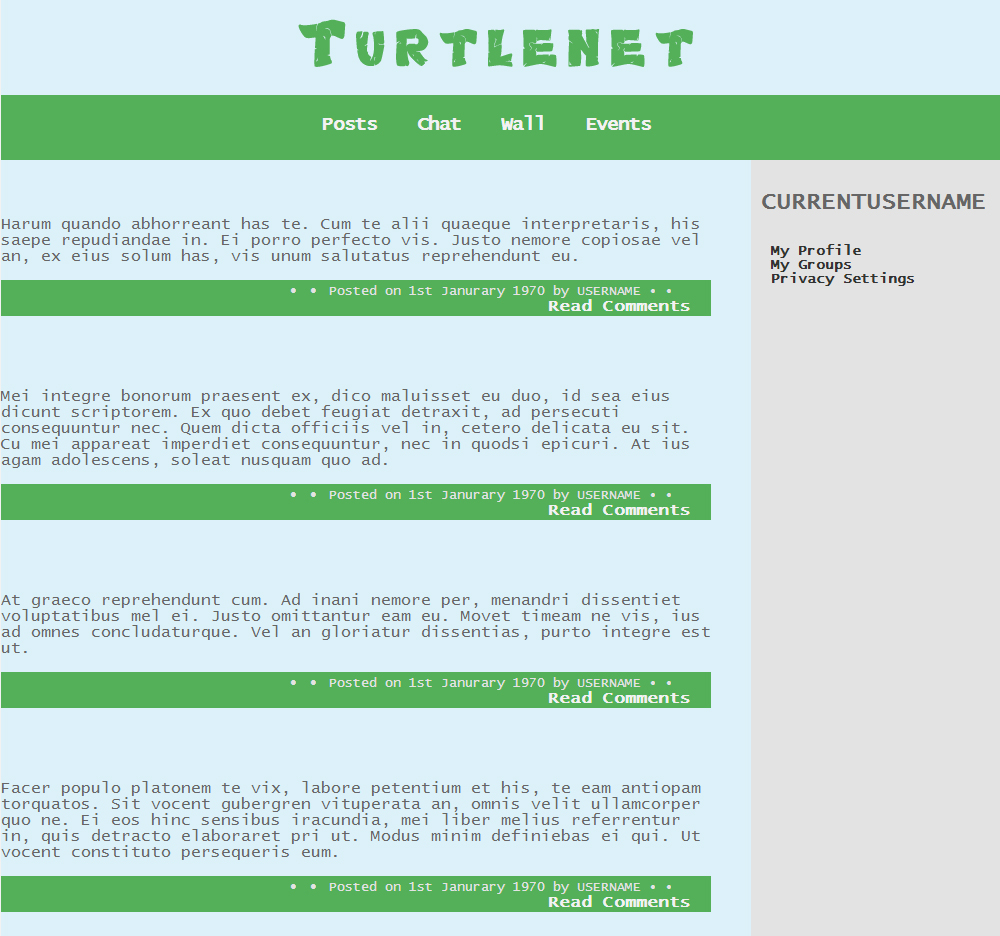
\includegraphics[width=\textwidth]{images/design/client_interface.jpg}
    \caption{Client Design Image}
    \label{fig:client}
\end{figure}

Most users will be familiar with HTML and CSS page layouts, even if they do not
know what HTML or CSS is. This will provide a certain level of comfort when it 
comes to using new applications and how to navigate between pages or tabs.

\subsection{Server Design}
Whilst not critically important, as it would only be operated by those with 
technical knowledge, is still an important aspect to consider. It needs to hold 
the system level settings and control mechanisms a server client would need, 
whilst not making them immediately and 'accidentally' accessible via the form of 
large obvious buttons. The easiest way of doing this is via a command input box 
beneath a chat log window to provide commands that way. It is also may be an 
idea to show server data such as memory usage on the operators end, as this data 
is completely accessible and non-intrusive to the client. The figure labelled 
'Server Design Image' shows an example of how the server client may be completed.
Pending on the features allowed in GWT, our method of choice, we will aim for 
it to retain a similar appearance.

\begin{figure}[h]
    \centering
    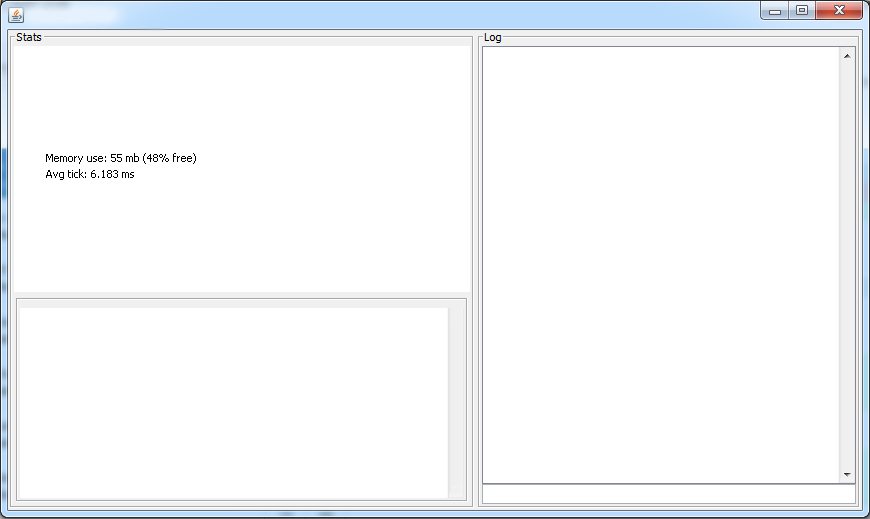
\includegraphics[width=\textwidth]{images/design/server.jpg}
    \caption{Server Design Image}
    \label{fig:server}
\end{figure}

\section{Future Work}
With some of the spare resources available during this phase, we were able to 
look into some future design work on the mobile front. One of our designers had
some experience in this field of work and offered to put some images together 
of what a mobile application version of our product could potentially look like. 

\begin{figure}[h]
    \centering
    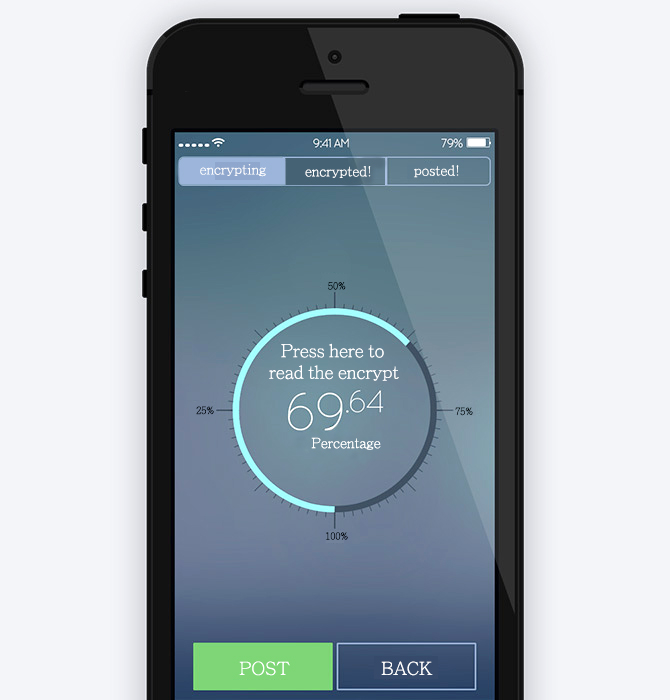
\includegraphics[width=\textwidth]{images/design/mobile_send.jpg}
    \caption{Mobile Sending Stage GUI}
    \label{fig:mobile_send}
\end{figure}

\begin{figure}[h]
    \centering
    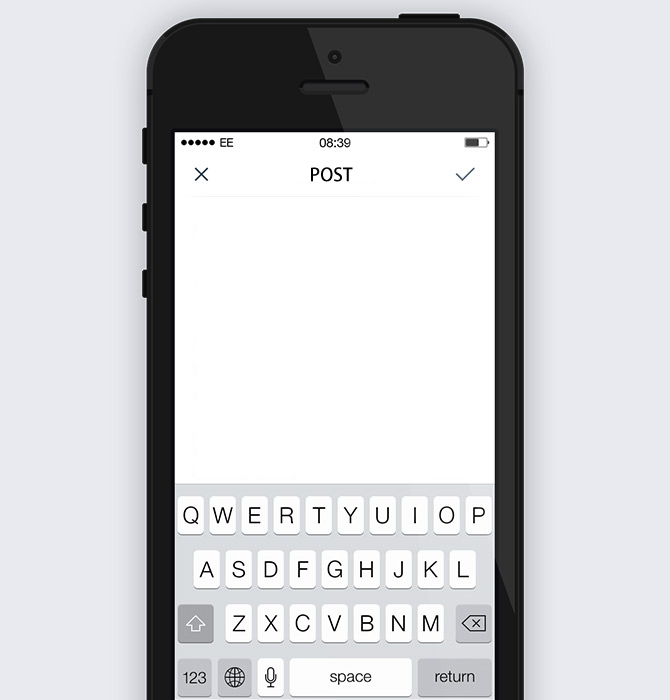
\includegraphics[width=\textwidth]{images/design/mobile_post.jpg}
    \caption{Mobile Post Stage GUI}
    \label{fig:mobile_post}
\end{figure}

The mobile interface data flow diagram shows how the application would flow 
between screens, giving an idea to the level of depth an application of this 
size might have.

\begin{figure}[h]
    \centering
    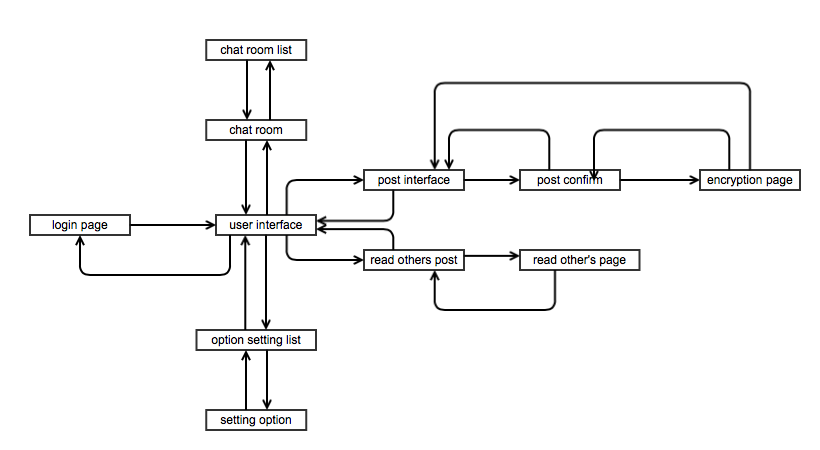
\includegraphics[width=\textwidth]{images/design/mobile_flow_diag.png}
    \caption{Mobile Data Flow Diagram}
    \label{fig:mobile_flow}
\end{figure}